
% This first part of the document. Here you declare the type of document and the size of the text along with the paper size.
\documentclass[a4paper,11pt]{article}
%This is the packages used. They allow to use additional commands to format the document.
\usepackage[utf8]{inputenc}
\usepackage{graphicx}
\usepackage[english]{babel}
\usepackage[vmargin=3.5cm, top=2cm]{geometry}
\usepackage[linktocpage=true]{hyperref}
\usepackage{enumitem}
\usepackage{longtable}
\usepackage{pdfpages}
\usepackage{float}
\usepackage{hyperref}
\usepackage[section]{placeins}
\usepackage{listings}
\hypersetup{
    colorlinks,
    citecolor=black,
    filecolor=black,
    linkcolor=black,
    urlcolor=black
}
%New commands declared. This allows for easier declarations.
\newcommand{\tmtable}{\begin{longtable}{ p{2.7cm} p{10cm} }}
\newcommand{\tmtableend}{\end{longtable}}

\begin{document}
\lstset{language=C}  

%This is the titlepage. Here you can format and declare the front page of the document.
\begin{titlepage}
%Centers the text and removes automatic indentation
\centering \parindent=0pt
\newcommand{\HRule}{\rule{\textwidth}{1mm}}
\vspace*{\stretch{1}} \HRule\\[1cm]\large\bfseries
Title of the project\\[0.7cm]
\large Thesis Project\\[1cm]
\HRule\\[1cm]


\large by 
\\Mikkel Stolborg (msto@itu.dk)
\vspace*{\stretch{2}} \normalsize
\begin{flushleft}
IT University of Copenhagen \\
Supervisor\\
Name of supervisor\\
\today \end{flushleft}
\end{titlepage}

\begin{abstract}
Here you write the abstract of the project. The reason for having it as an abstract command section, is to not include it in the page count.
\end{abstract}
%breaks to next page.
\pagebreak
%Generates the table of content from the sections headings.
\tableofcontents
\pagebreak
\section{Section}
A section is the top level of document. The structure goes section, subsection, and subsubsection.

The figure, a simple Image, can be referenced by its label. The figure \ref{fig:simpleImage}, will be the simple image.

\begin{figure}[h]
    \centering
    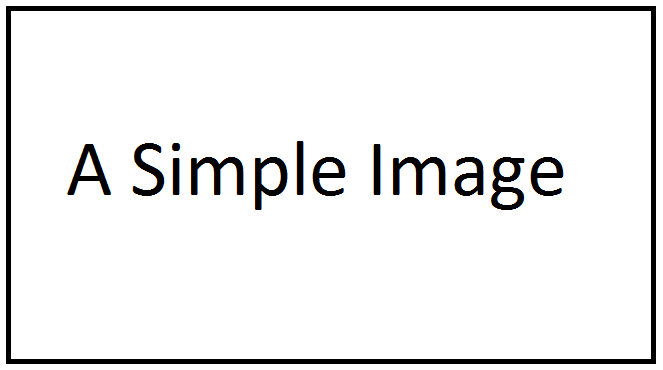
\includegraphics[width=0.8\textwidth]{Images/SimpleImage.png}
    \caption{This is the caption of the image. The figure is placed as close as possible to the text above. This is determined by the [h] command at the figure. The image is 80\% of the text width as given above. The image is located in a subfolder, as given in the path.}
    \label{fig:simpleImage}
\end{figure}

\subsection{Subsection}
\subsubsection{Subsubsection}

\begin{table}
	\begin{tabular}{|l|l|}
		\hline
		Table name & column name\\ 
		\hline
		Human Development Index & Name \\
		and its components & 2012 Life Expectancy at Birth\\
		& 2010 Mean Years of Schooling\\
		\hline
		Gender Inequality Index & 2012 Gender Inequality Index Value\\
		& 2010 Maternal Mortality Ratio\\
		& Adolescent Fertility Rate\\
		& 2012 Seats in National Parliament (\% female)\\
		& 2006-2010 Population with at least secondary education (Female)\\
		\hline
		Command over resources & 2011 GDP\\
		& 2005-2010 Education \% of GDP\\
		& 2010 Military \% of GDP\\
		\hline
		Health & 2009 Adult Mortality Rate - Female\\
		& 2009 Adult Mortality Rate - Male\\ 
		\hline
		Education & 2010 Population with at least secondary education\\
		& 2009 Mathematics Mean Score\\
		& 2009 Science Mean Score\\ 
		& 2009 Reading Derivation from Mean\\
		\hline
		Social integration & 2011 Employment to Population Ratio\\
		& 2005-2011 Youth Unemployment\\
		& 2007-2011 Trust in National Government\\
		\hline
		International trade flows & 2010 Exports of merchandise goods (\$ Billions)\\
		of goods and services & 2010 Imports of merchandise goods (\$ Billions)\\
		& 2010 Exports of services (\$ Billions)\\
		& 2010 Imports of Services (\$ Billions)\\
		& 2010 Agricultural Share of Merchandise Exports\\
		& 2010 Manufactured Share of Merchandise Exports\\
		& 2010 Agricultural Share of Imports \\
		& 2010 Manufacutured Share of Imports \\
		\hline
		International capital & 2007-2011 Total reserves minus gold\\
		flows and migration & 2010 International inbound tourism\\
		\hline
		Innovation and technology & 2002-2010 Research and Development Researchers\\
		& 2002-2011 Graduates in Science and Engineering\\
		& 2002-2009 Personal Computers\\
		& 2010 Internet Users\\
		\hline
		Environment & 2009 Fossil Fuel Usage\\
		& 2009 Renewable Energy Usage\\ 
		& 2008 Carbon Dioxide Emissions\\
		& 2010 Forest Area\\ 
		& 2011 Endangered Species\\
		& 2009 Agricultural Land\\
		\hline
		Population trends & 2012 Population\\
		& 2012 Urban Population\\
		& 2010 Median Age\\
		\hline
	\end{tabular}
	\caption{The selected tables data and selected columns}
	\label{Tab:dataSelect}
\end{table}

\begin{equation}
	y = \alpha \times x -\beta
	\label{func:function}
\end{equation}

\bibliography{sources}{}
\bibliographystyle{plain}



\end{document}
